%\pagebreak
\section{Measurement setup}

Once the experimentalist has deemed their sample worthy of measuring, there are a few battles to be fought to connect the sample fabricated in the cleanroom and to the electric equipment in the measurement laboratory.

\subsection{Device packaging}\label{sec:fab-packaging}

% 
After the device fabrication is finished, the sample has to be mounted on a chip carrier and contacted, so we can connect it to our measurement electronics.
% 
Our microwave PCBs are made for \SI{10x10}{\milli\meter} chips; however in order to grab the chips during fabrication easier and to enhance the fabrication yield, samples are usually fabricated on larger substrates:
% 
The current bias cavities for the graphene devices presented in this thesis were processed on a \SI{2}{inch} wafer, and the cavities based on aluminum on \SI{15x15}{\milli\meter} chips.

We dice the chips into the correct dimensions as the very last step, using the \textit{Disco dicer} DAD 3220 from \textit{Disco Hi-Tec Europe GmbH}.
% 
To protect the chip from dust during sawing, we spincoat photoresist\footnote{HPR504, \SI{4000}{rpm}, bake \SI{60}{\second} at \SI{100}{\celsius}, approximately \SI{1.2}{\micro\meter} thick} on the chip before dicing.
% 
Good resist-substrate adhesion is important during dicing because the water jet used to cool the blade can wash off the resist during dicing otherwise, potentially ruining weeks of delicate work in the cleanroom.
% 
Use of HMDS, or letting the resist sit on the chip to be diced for \SI{1}{\minute} prior to spinning is highly recommended.

The silicon chips were diced using a standard NBC blade at \SI{3000}{rpm} and a feed speed of \SI{5}{\milli\meter\per\second}, while for dicing sapphire we used a special diamond blade at \SI{2000}{rpm} and \SI{2}{\milli\meter\per\second}.
% 
Removing the protective resist after dicing can depend on the device materials.
% 
For the devices presented in this thesis, we placed the diced chips in teflon holders inside beakers filled with PRS3000, heated the solution to \SI{80}{\celsius} and subsequently put the beaker into an ultrasound bath at maximum power.
% 
After \SI{5}{\minute}, the resist has then come off the sample, and we passed the chip through a series of PRS3000 and IPA baths to wash off any remains, and blow-dried using nitrogen.

% 
The chips are finally glued to the rails of our copper boxes using GE low temperature varnish.
% 
Wirebonding is done using a \textit{Westbond 4000 "E"} system from \textit{West•Bond Inc.} with bond wires from an AlSi alloy (\SI{99}{\percent}-\SI{1}{\percent}).
% 
To ensure good thermalization and electrical contact, we usually used three to four bonds for each bond pad, and as many bonds as would fit on the ground planes.
% 
An example of one of our devices that is mounted and wirebonded in a PCB, ready for measurement can be seen in Fig.~\ref{fig:packaging}.
% 
The connectors to go from the PCB to the outside world are straight plug semi-detent SMP connectors\footnote{19S102-40ML5 straight plug PCB, from \textit{Rosenberger Hochfrequenztechnik GmbH \& Co. KG}}.


\begin{figure}
	\centering
	\includegraphics{{chapter-experimental-methods/figs-packaging/packaging.svg}.png}
	\caption{
		\textbf{Device packaging for electrical measurements.}
		% 
		\textbf{A,} A \SI{10x10}{\milli\meter} mounted and wirebonded to a PCB, that is screwed onto a copper base.
		% 
		The four small holes around the chip are used to screw on a small copper lid, covering the chip.
		% 
		The four big holes at the edge of the copper based are used for mounting the chip in a cryostat, and to hold the top cover in place.
		% 
		Connectors for connecting the PCB to the outside world are surface mount SMP plugs.
		% 
		\textbf{B,} Close-up of the bottom-right chip area, taken with ring illumination.
		% 
		The substrate is sapphire, hence the chip transparency.
		% 
		In the bottom right corner, one of the copper rails on which the chip sits is visible.
	}
	\label{fig:packaging}
\end{figure}

\subsection{Thermal energy and noise}

Temperature means that there are available excitations at a given energy, corresponding to a (thermal) frequency
\begin{align}
f_{th}=\frac{k_B T}{h}.
\end{align}
Below we give the thermal energies and frequencies corresponding to typical temperatures in our setups:
\begin{center}
\begin{tabular}{ccc}
	\hline \hline
	Temperature & Thermal frequency & Thermal energy \\ 
	\hline 
	\SI{300}{\kelvin} & \SI{6.25}{\tera\hertz} & \SI{25.9}{\milli\electronvolt} \\ 
	% \hline 
	\SI{50}{\kelvin} & \SI{1.04}{\tera\hertz} & \SI{4.3}{\milli\electronvolt} \\ 
	% \hline 
	\SI{4}{\kelvin} & \SI{83.3}{\giga\hertz} & \SI{345}{\micro\electronvolt} \\ 
	% \hline 
	\SI{100}{\milli\kelvin} & \SI{2}{\giga\hertz} & \SI{8.62}{\micro\electronvolt} \\ 
	% \hline 
	\SI{10}{\milli\kelvin} & \SI{208}{\mega\hertz} & \SI{862}{\nano\electronvolt} \\ 
	\hline \hline
\end{tabular}
\end{center}

In order to neglect the influence of thermal effects on our circuits and for the superconductor to be in its thermal ground state, it is absolutely necessary to operate the devices at temperatures $T \ll T_c$.
Since the superconducting gap voltages of \ce{NbTiN}, \ce{MoRe} and \ce{Al} are \SI{2.3}{\milli\electronvolt}, \SI{1.5}{\milli\electronvolt} and \SI{183}{\micro\electronvolt}, respectively, our experiments require access to the sub-Kelvin regime which is enabled by using dilution refrigerators.

However, even with thermal excitations suppressed by thermally anchoring our devices to the millikelvin stages of our dilution refrigerators, thermal noise from our setup propagating through the electrical connections necessary to probe our devices, can induce unwanted excitations which can severely hinder experiments.
The amplitude of such thermal noise current, voltage and power of a resistor are
\begin{align}
I_n &= \sqrt{\frac{4k_B T\Delta f}{R}} \\
V_n &= \sqrt{4k_B T R\Delta f} \\
P_n &= k_B T \Delta f \\
P_{dBm} &= 10\log_{10}(k_B T\Delta f)+30
\end{align}

For a measurement bandwidth of \SI{1}{\hertz} and a resistor of \SI{50}{\ohm}, this corresponds to the following values for temperatures typically used in our setup:

\begin{center}
\begin{tabular}{cccc}
	\hline \hline
	Temperature (\si{\kelvin}) & Noise power (\si{dBm}) & Noise voltage (\si{\pico\volt}) & Noise current (\si{\pico\ampere})\\ 
	\hline 
	300 & -174 & 910 & 18 \\ 
	% \hline 
	50 & -182 & 372 & 7 \\ 
	% \hline 
	4 & -193 & 105 & 2 \\ 
	% \hline 
	0.1 & -209 & 16.6 & 0.3 \\ 
	% \hline 
	0.01 & -219 & 5.3 & 0.1 \\ 
	\hline \hline
\end{tabular}
\end{center}

Moreover, current and voltage fluctuations originating from room temperature electronics can carry the typical \SI{50}{\hertz} interference (also dubbed \textit{mains hum}), along with other, high-frequency, components.
In our lab, we suppress the mains hum by physically separating any electronic equipment powered by the \SI{50}{\hertz} power system from our DC electronics.
Our DC electronics, the IVVI rack, is home-made at \textit{DEMO}\footnote{Dienst Elektronische en Mechanische Ontwikkeling, \url{https://www.tudelft.nl/demo/}} of TU Delft.
\begin{itemize}
	\item 50 Hz
	\item other sources of electronic noise
	\item battery powered and separated grounds, including measurement?
	\item low pass filters
\end{itemize}

The detailed recipe for making the copper powder filters can be found in appendix \ref{app:copperpowder}.

\begin{figure}
	\centering
	\includegraphics[]{{chapter-experimental-methods/figs-setup/noise_filter.svg}.png}
	\caption{
		\textbf{Electronic noise reduction using low-pass filters.}
		\textbf{A,} Measured transfer function of individual homemade copper powder and two-stage RC filters.
		The cut-off frequency for the RC filters is approximately \SI{30}{kHz}, while high-frequency noise leaks through above \SI{20}{MHz}.
		The copper powder filters significantly suppress frequencies above \SI{100}{MHz} and above.
		\textbf{B,} Photograph of a two-stage RC filter of SMD 0812 elements and a fully assembled copper powder filter.
		Inset, copper powder filter PCB with connector, without enclosure.
		The PCB trace is approximately \SI{50}{\centi\meter} long.
	}
	\label{fig:filter}
\end{figure}

\subsection{Fridge wiring}

\begin{figure}
	\centering
	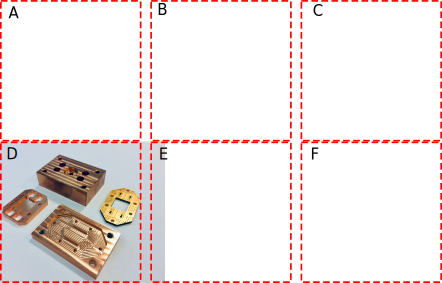
\includegraphics[]{{chapter-experimental-methods/figs-packaging/wiring.svg}.png}
	\caption{
		\textbf{Cryogenic fridge wiring.}
		\textbf{A,} Inside view of a Bluefors LD dry dilution refrigerator.
		\textbf{B,} Photograph of a four-port PCB mounted on a copper block with rails.
		\textbf{C,} Fully enclosed sample mounted inside of a hand-wound magnet and bolted to the millikelvin stage of the dilution refrigerator.
	}
	\label{fig:wiring}
\end{figure}

All measurements presented in this thesis were performed at millikelvin temperatures, using dry dilution refrigerator models \textit{Triton} from \textit{Oxford Instruments} or \textit{LD-400} from \textit{Bluefors Oy}.

\begin{itemize}
	\item noise temperature calculation a la Bluefors
	\item pictures
\end{itemize}

